% using Elseveir template per https://www.elsevier.com/authors/author-schemas/latex-instructions
% model paper: Dynamic effects of teacher turnover on the quality of instruction (2016)
%   Hanushek et al
%   from Economics of Education Review

% secondary model paper: The effects of economic policy and political uncertainties on economic activities
% Gholipour, 2019
% https://www.sciencedirect.com/science/article/pii/S0275531918306081
\documentclass[review]{elsarticle}

\usepackage{lineno,hyperref}
\modulolinenumbers[5]

\journal{Journal of \LaTeX\ Templates}
\bibliographystyle{elsarticle-num}
\usepackage{booktabs}
\usepackage{graphicx}
\graphicspath{{../alt-ed-survey/figures-and-tables}}
\usepackage{hyperref}
\usepackage{threeparttable}  
\usepackage{tikz}
\usetikzlibrary{calc,matrix}

\begin{document}

\begin{frontmatter}

\title{
    Dynamic Effects of H-1B and Section 127 Policy Interaction on Higher Education
    \tnoteref{titlenotes}
}
% \tnotetext[titlenotes]{
%     Go to \url{https://github.com/Vandivier/research-dissertation-case-for-alt-ed/tree/master/papers/}
%     for additional materials including the online appendix,
%     survey data, and data analysis source code.
% }

\author[mymainaddress]{John Vandivier} % \fnref{authorlinefootnote}}
\address[mymainaddress]{4400 University Dr, Fairfax, VA 22030}
\ead{jvandivi@masonlive.gmu.edu}

\begin{abstract}
    % role model abstract based on Hanushek et al (2016)
    % model length = 151 words
    % this abstract length = 165 words
    % narrative-problem-solution structure
    % ---
    It is widely believed that employer educational assistance increases the quantity demanded for higher education,
    but the original passage of Section 127 which enables this tax-deduction for employers is associated with a reduction to the growth of higher education enrollment,
    and a simple regression of the assistance limit on total enrollment indicates a significant negative correlation. % technically, `reg totalen emp' in my data set
    This raises concerns that confounding factors bias estimates of the effectiveness of Section 127 assistance.
    After taking extensive steps to account for policy effects and other dynamic economic factors,
    I robustly identify a positive effect on enrollment from employer educational assistance
    by exploiting real variation in employer educational assistance over the 27-year period from 1990 to 2016.
    Results are validating using panel vector autoregression (PVAR),
    dynamic least squares (DOLS) methods,
    and instrumental variable (IV) approaches.
    In the preferred model,
    an increase in tax-deductable employer educational assistance
    in the amount of one dollar is associated with
    an increase of about 600 to national total enrollment in institutions of higher education.

    % Highlights
    % 1. Section 127 Employer Assistance
    % 2. 
    % 3. 
    % 4. 

    % % alternate role model abstract based on Gholipour
    % % model length = 129 words
    % % this abstract length = 91 words
    % % technical micropaper structure
    % % ---
    % This paper explores the dynamic effects of Section 127, veteran education benefits, Stafford loan, and H-1 Visa policy
    % on total enrollment in the United States
    % using annual data from degree-granting institutions in the United States during the 27-year period from 1990 to 2016.
    % By applying panel vector autoregression (PVAR) and dynamic least squares (DOLS) methods,
    % the results show that a positive shock to Section 127 assistance triggers a positive response from enrollment in the short-run.
    % In addition, I find that higher levels of assistance do not significantly decrease enrollment in the long-run.
\end{abstract}

\begin{keyword}
education economics, section 127, educational assistance, veteran education, h-1b, debt crisis, dols, vars
\MSC[2010] % TODO
\end{keyword}
\end{frontmatter}

\pagebreak
\linenumbers

    \section{Introduction}

    % background scratch notes in this comment block:
    % degree requirement as a strategy to import cheap, effective foreign labor (VISA)
    % this prevents high school graduates from directly entering roles that typically award section 127 (white color, major employer, corporate work)
    % until recently, that is, with walmart, mcdonalds, starbucks giving section 127 i think even to part timers
    % Theory: After 1990, companies began requiring a 4 year degree so they could have an H-1B justification.
    % This caused more americans to pursue an undergraduate degree without section 127. we should see section 127 use decline after 1990.
    % Revisit in conclusion -> Recently, employers have begun giving the benefit anyway due to labor selection and internal ROI benefits

    Basic supply and demand theory indicate that a reduction in price is associated with an increase to the quantity demanded.
    In 1978, a bill was passed allowing employer educational assistance to be tax-deductable in the United States up to a nominal limit of 5,000 dollars.
    It is surprising, therefore, that 1978 is associated with a local decrease in the growth rate on both total and public university enrollment.
    This study exploits real variation in the tax-deductable employer educational assistance limit to eventually identify the expected positive effect,
    but not before identifying and correcting for several interesting things going on in the economy.
    Specifically, an interaction between H-1B policy and Section 127 employer educational assistance is discovered and assessed.

    \subsection{Supply-Side Explanations}
    Before forming more exotic theories, some simpler hypotheses should be checked.
    One hypothesis is that there is an adjustment period after the passage of Section 127 and before widespread employer provision of the newly deductable benefit.
    Allowing for a 3 or 5 year lag around the passage of Section 127 in 1978 does not resolve the issue.
    Across the eight five-year periods from 1970 to 2010, the five-year public enrollment growth rate was above 9 percent as often as it was below.
    Two of the four low-rate intervals occured immediately subsequent to the 1978 creation of Section 127.
    The interval just prior, from 1970-1975, saw the highest growth in enrollment across the period.
    It does not appear to be a one-year fluke that the employer educational assistance is associated with declined enrollment growth.
    
    Another important point is that Section 127 was passed in 1978, but it took effect in the 1979 tax year.
    1979 saw modest growth in enrollment,
    but given the pre-existing long-run context of positive trend in enrollment,
    it is not clear that Section 127 can be attributed any causality.

    An alternative to the 3 or 5 year lagged analysis is to directly refer to surveys of employers.
    Cappelli\cite{cappelli2004employers} identifies 3 employer surveys from 1992 and 1993 which indicate that at least 86 percent of surveyed employers provided educational assistance.
    These studies were samples of convenience with a focus on large employers,
    but additional information leads Cappelli to claim that a substantial majority of employers offer such plans over his period of analysis from about 1990 to 2004.
    Cappelli notes that employee utilization of the benefit favors graduate education
    with about 20 percent of graduate students receiving employer assistance
    and roughly 6 percent of undergraduates doing so.
    Common provision of the benefit has remained true in later years.
    In 2013, SHRM reported that 61 percent of employers offer tuition assistance\cite{cherry2014rejuvenating}.
    In 2017, World at Work found that 85 percent of employers offered such a benefit,
    with another 7 percent offering non-reimbursement tuition assistance, such as upfront tuition discounts\cite{talentculture_2018}.

    \subsection{H-1B, Veteran Education Benefits, and Stafford Loan Interaction}
    The idea that graduate students mainly use employer education benefits motivates hypotheses around undergraduate access.
    Increasingly since the 1990s, developed economies have experienced degree inflation and experience inflation.
    Entry level positions now require a degree when previously this was not necessary, even when technology has made the work easier.
    It is possible that undergraduate access to employer benefits are reduced simply because employers increasingly hire individuals that already have the degree.
    Employers are known to value the degree as a signal of labor quality, but these days there are plenty of other, richer data sources on quality for certain professions.
    In computer programming we see some employers completely dropping the degree requirement and preferring technical interviews, digital portfolio evaluation, and other signals.
    Why, then, do other leading employers continue to require the degree?
    One answer is that the degree requirement forms an H-1B justification.
    Since the passage of the Immigration Act of 1990\cite{law1990law}, a corporation must claim a shortage of qualified specialized labor to justify an H-1B.
    The "attainment of a bachelor's or higher degree" is written into the law as a test of whether labor is qualified and specialized.
    This would motivate employers to begin requiring the degree in order to obtain cheap immigrant labor, even while knowing the degree may not be necessary.

    Zero employers offered Section 127 educational assistance in 1977, but the majority offered the benefit by 1993.
    Immigration policy is a change which interrupts this period of analysis, but there are two other major policies to take note of.
    Stafford loans were available before Section 127, but the limits and rules for these loans and other government assistance to higher education fluctuated over the period of analysis.
    Government educational benefits for veterans is another major policy in the higher education assistance space.
    It becomes difficult to imagine a proper Section 127 analysis which does not include dynamic correction for these potentially important factors,
    as well as correction for general price changes and economic conditions in the economy over time.
    Such a corrected analysis is exactly what this paper completes.

    \subsection{Demand-Side Explanations}
    The prior explanations consistitute a supply-side exploration of the impotence of Section 127.
    An alternative explanation is that there simply wasn't much demand for college in the early years of Section 127.
    Indeed, lack of market demand appears to be a good explanation for the consistent college-age enrollment percent
    which is observed at 25.7 percent in both 1970 and 1980.
    A demand-side explanation is consistent with the falling average tuition and fees observed for all institutions from 1972 to 1980.
    After 1980 we see an upward trend in price and also an upward trend in college-age enrollment percentage, as well as simple total enrollment.

    With an increase to the Stafford limit in the 1977 school year,
    a major change to veteran education benefits in the 1981 school year,
    Section 127 beginning in the 1978 school year,
    and price changes in higher education and for all other goods,
    claims about a particular cause become dubious without full and corrective statistical treatment.
    Even so,
    there is some plausibility to the claim that Section 127 was passed during a time when demand was weak,
    so that there may have been a positive effect on the part of Section 127 as early as the first year,
    but it was overshadowed by general decline.
    The main contribution of this line of thought to a more general analysis is that corrective statistics should include price data
    for education in particular, and also for the general economy.

    \section{Empirical Model}

    Equation \ref{eq1} is an ordinary least squares model of total enrollment higher education in the United States.

    \begin{equation}
        Y = \beta_1X_1+\beta_2X_2...+\beta_kX_k+e
        \label{eq1}
    \end{equation}

    The Section 127 policy effect is the variable of interest.
    Three other policy variables are included for federal lending policy, veteran education benefits, and H-1 Visa policy.
    In addition to the four policy variables, 
    enrollment is modelled as a function of time,
    and the price of tuition and fees.
    A variable for personal consumption expenditures (PCE) as an measure of inflation is also included.

    For robustness and analytical completeness, I test two other left hand variables using ordinary least squares,
    then I also test the relation of interest with two other modelling approaches.
    Specifically, I explore vector autoregressive (VAR) models
    and an instrumental variable regression following the Anderson–Hsiao pattern\cite{anderson1981estimation} with the lagged variable of interest as an instrument.

    \section{Data}

    Information on total enrollment for all degree-granting postsecondary institutions in the United States
    is provided by the National Center for Education Statistics (NCES)\cite{nces_2019}.
    Enrollment figures are for the fall semester of the school year.
    Information on selected years from 1947 to 2028 is provided, where values for 2018 and later are projected.
    The present study does not use any of the projected values.
    Other data sources and policy considerations constrain the period of interest to the 27-year period from 1990 to 2016.    
    % total enrollment: https://nces.ed.gov/programs/digest/d18/tables/dt18_303.10.asp

    Personal Consumption Expenditures (PCE) data is a measure of inflation provided by the U.S. Bureau of Economic Analysis (BEA)\cite{bea_2020}.
    Education-specific inflation is also calculated using NCES data\cite{nces_2017}.
    NCES data is the average tuition and required fees for full-time undergraduate students across all degree-granting postsecondary institutions.
    NCES provides nominal values and values adjusted for the consumer price index (CPI) for tuition.
    The price of room and board is ignored.
    % https://fred.stlouisfed.org/series/PCE
    % https://nces.ed.gov/programs/digest/d17/tables/dt17_330.10.asp

    Nominal Section 127 limits are a matter of public law.
    Section 127 took effect beginning after December 31, 1978 with a nominal assistance limit of 5,000 dollars\cite{plaw95_600_1978}.
    In October 1986, Pub. L. 99–514 increased the nominal assistance limit to 5,250 dollars\cite{plaw99_514_1986}.
    Real Section 127 employer assistance limits are calculated two ways.
    One variable is constructed for each measure of inflation.
    Price deflators for each measure of inflation use 2016 as a base year.
    
    % begin discuss veteran benefits data
    Changes to veteran education benefits are also a matter of public law.
    A categorical variable is used to capture the state of veteran education benefits among five possible states over the period from 1970 to 2020.
    The Servicemen's Readjustment Act of 1944,
    also called the G.I. Bill,
    is the first interesting case of veteran benefits,
    but it precedes the period of interest for this study.

    The original bill expired in 1956\cite{glass_2010}.
    This expired state is the first state represented by the veteran education state variable.
    The Veterans Educational Assistance Program (VEAP) was established in 1981\cite{veteransaffairs_2017}.
    A third period of interest begins in 1984 with the enactment of the Montgomery GI Bill\cite{powers_2018}.
    A fourth period of interest begins in 2009 with the Post-9/11 GI Bill.

    Finally, many benefits from the Forever GI Bill became effective in 2018,
    with additional provisions taking effect in 2020 and 2022\cite{veteransaffairs_2020}.
    This fifth policy state is too recent to be included in the period of interest.
    The recent changes in veteran education benefits are a critical caveat for any attempt at forecasting or prediction outside of the period of study.

    Due to constraints on the availability of other right hand variable data,
    the main period of regression analysis ranges from 1990 to 2016.
    Veteran education benefits exhibit only one change during this period,
    but this factor proves to be significant in the preferred model.
    % GI Bill accounting https://en.wikipedia.org/wiki/G.I._Bill#Chapter_30_(Montgomery_GI_Bill)
    % Variable implemented as categorical
    % [state A] original bill was 1944-1984
    % [state B] VEAP established 1981 https://www.benefits.va.gov/gibill/veap.asp
    % [state C] Montgommery GI went into effect 1984
    % [state D] Post-9/11 GI Bill went into effect for 2009 school year https://www.thebalancecareers.com/gi-bill-for-the-21st-century-3347143
    % [state E] Forever GI bill rolls out new benefits starting in 2018 https://rebootcamp.militarytimes.com/education-transition/education/2017/08/16/trump-signed-the-forever-gi-bill-here-are-11-things-you-should-know/
    %
    % end discuss veteran benefits data

    Stafford loan data is another key component of the analysis.
    Stafford loan data is directly relevant by itself,
    but it is further intended a proxy for broader non-military federal student aid policy.
    There are two variables for Stafford loans.
    The first is the nominal loan limit for undergraduates.
    The second is a dummy variable indicating whether the undergraduate loan limit
    is the combined limit for undergraduate and graduate loans.
    A policy change became effective in 1993 which grouped these limits together.
    Stafford loan data is sourced from FinAid\cite{finaid_2020}.
    % TODO: should I dive into an explanation for focus on undergraduate education? not doing for now.

    Visa policy is a complex issue.
    Annual H-1B visa award is an important and simple variable used for the purposes of this study.
    The Immigration Act of 1990 decomposed the existing H-1 visa into distinct H-1A and H-1B categories.
    Over time, H-1B1 and H-1C classifications were established,
    and many other important but less relevant classifications outside of the H-1 family exist as well.
    The H-1B visa is most relevant for this study because it specifically relates to the undergraduate degree.
    The Immigration Act of 1990 makes available the H-1B classification for specialized workers,
    or workers in a specialty occupation.
    A specialty occupation is formally defined as "an occupation that requires...attainment of a bachelor's or higher degree..."

    H-1 visas are a subgroup of nonimmigrant visas.
    Nonimmigrant visa award data by classification from 1987 to 2019 is provided by
    the Bureau of Consular Affairs within the United States State Department\cite{bureauof_2020}.
    This paper exclusively uses the most relevant H-1B visa award numbers,
    but reanalysis with other visa classifications could yield statistically significant findings.
    The prior H-1 visa was also a merit worker visa, but it had no formal definition of merit.
    In 1989, 48,820 H-1 visas were awarded.
    In 1991, 7,443 H-1A visas were awarded, and 51,882 H-1B visas were awarded.
    It's plausible that the college-educated effect informally existed prior to the 1990 legislation.
    One might also find small but significant effects by looking into visas outside the H-1 family.
    Besides the number of actual visa awards, an analyst could look for visa cap effects,
    or visa policy state effects.
    For example, Pew Research Center notes that the American Competitiveness in the 21st Century Act of 2000 exempts certain entities from the H-1B cap\cite{ruiz2017key}.
    % ref: https://en.wikipedia.org/wiki/H-1B_visa#H-1B_visas_issued_per_year
    % more state variable food https://redbus2us.com/h1b-visa-total-cap-history-from-1990-to-current-year/
    % 1952 allows unlimited merit immigration, 1990 there is a quota and degree requirement added to H-1B: https://en.wikipedia.org/wiki/H-1B_visa#Immigration_Act_of_1990
    % A crackdown in 2017: https://www.investopedia.com/news/impact-trumps-h1b-visa-crackdown-5-charts/
    % other policies for policy state analysis:
    %   https://en.wikipedia.org/wiki/Legal_Immigration_Family_Equity_Act#V_visa
    %   not sure it's relevant - https://en.wikipedia.org/wiki/Immigration_Reform_and_Control_Act_of_1986
    %   https://en.wikipedia.org/wiki/H-1B_Visa_Reform_Act_of_2004
    %   1986 we get h-2a and h-2b https://www.uscis.gov/ilink/docView/AFM/HTML/AFM/0-0-0-1/0-0-0-13593/0-0-0-13614.html
    %   more 1986 context https://www.vox.com/2014/9/3/18080710/immigration-immigrants-reform-us
    %   various visa info https://uk.usembassy.gov/visas/temporary-employment/petition-based-visas/
    % 
    % Open SE questions looking for more data:
    % 1) https://politics.stackexchange.com/questions/52279/us-pre-1987-visa-issue-data
    % 2)
    % 
    % Open Tweet looking for more data:
    % https://twitter.com/JohnVandivier/status/1243975718649974786
    % apparantly official response via twitter...cite if you dare: https://twitter.com/TravelGov/status/1243985245382283266
    % they daring me: https://academia.stackexchange.com/questions/119549/can-a-tweet-be-added-to-graduate-research-proposal
    % "with the caveat of ambiguous language,
    %   the State Department appears to confirm tha pre-1987 data is currently digitally unavailable,
    %   and perhaps permentantly unrecorded even offline."

    The last data source of interest is on actual federal loans.
    Actual federal loans stand in contrast to loan limits which are represented by the Stafford loan limit variable.
    Loan limits are a policy choice, but after correcting for loan limits the actuals primarily represent a demand effect.
    As such, we would not want to correct for actual loans.
    That would wipe out the effect of interest,
    which is the demand effect attributable to various policies,
    and Section 127 employer educational assistance in particular.

    Instead, loan data is taken as a left hand variable of secondary interest.
    Section 127 is taken as a right hand variable in that brief investigation.
    This allows us to briefly review the relationship between Section 127 employer assistance
    and the student debt crisis, a potentially related topic of importance.
    The variable I use in this regard is total federal undergraduate loans,
    which is extracted from a worksheet labeled "Table 2_UG" in a data set provided by College Board\cite{cb_excel_2019}.
    Given additional context provided by The College Board in a related report\cite{cb_trends_2019},
    it is plausible that a seperate analysis which decomposes decomposing aggregate total federal loans by type of loan may yield marginal statistical improvement.
    % actual undergrad loans awarded since 1990 in the excel at https://research.collegeboard.org/trends/student-aid
    % My variable `Total UG Federal Loans` adapted from CB xlsx worksheet `Table 2_UG`

    \section{Results}

    The key independent variable is H-1B visa issuance, but at the outset there are two potential left hand variables available.
    % In simple regressions, H-1B effects are marginally more closely related to public enrollment compared to total enrollment.
    Ordinary least squares (OLS) multiple regression of visa effects, time, and tuition was run against both total enrollment and public university enrollment.
    Total enrollment was more predictable overall, so this was selected as the preferred enrollment variable.

    With total enrollment as the explained variable,
    a kitchen sink multiple regression was used to select the strongest factors among other factor groups.
    The total number of visas issued across classification is not significant.
    The long regression of interest has higher unadjusted explanatory power compared to kitchen sink regression.
    Measures of tuition were identified as insignificant.
    Table 1 is a table of regressions which helps illustrate that, somewhat surprisingly,
    real measures of employer assistance capture price and inflation effects in a preferred way
    compared to using a more direct measure of tuition.
    
    % \begin{table}
    %     \caption{Medium and Strong Models, Selected Variables}
    %     \begin{tabular}{lllll}
    %     Factor & 2018 Medium & 2018 Strong & 2019 Medium & 2019 Strong \\
    %     \toprule
    %     Male &  &  & -2.458* & -0.422** \\
    %     Not STEM & -1.269* \\
    %     X$_0$ & 1105.125 & .106 & -12345.347* & 3.289*** \\
    %     \bottomrule
    %     R-Squared & .597 & .504 & .526 & .319 %
    
    %     \end{tabular}
    %     \begin{tablenotes}
    %         \item{
    %             * p $<$ .05
    %             ** p $<$ .01
    %             *** p $<$ .001
    %         }
    %     \end{tablenotes}
    %     \label{tab:models}
    %     \end{table}



    H-1 visa effects, on the other hand, are highly significant and complex.
    All H-1 visa issuance factors are significant with p < .1.
    Somewhat surprisingly, the total number of visas issued within the H-1 family is more significant than the

    Section 127 assistance limits which are deflated using education-specific prices were identified as less significant
    compared to PCE-deflated Section 127 assistance.
    PCE remained important as a distinct variable.
    
    This makes some sense is in the context of a multiple regression.
    PCE and other factors already represent effects from inflation.
    While Section 127 asssistance deflated for education-specific inflation was identified as insignificant,
    nominal tuition seems to represent the same education-specific price information.




    1. > .995 adjusted r2 for preferred ols model
    2. empassist has positive coefficient in the range of 150-850; preferred measure around 600
    3. visa effects are complex and important, but signing the effect is sensitive to specification
    4. stafford and gi bill effects are also significant in the prefered model.

    % subsection: Factor analysis for education cost and inflation
    I also tested PCE as a distinct independent variable.
    In neither case did PCE present as a significant factor.
    The second approach turned out to be more significant
    \footnote{
        % TODO: Footnote [or optional table] comparing p-values for:
        % 1. reg VOI PCECORRECTION ALL_INSTITUTION_CORRECTION [with and without pce as seperate var]
        % 2. [optional] min p-value during round-robin process
    }.

    % TODO: maybe discuss Is H1 Edge Case variable...but is it significant? if not then not worth mentioning
    %   if it is significant then it means period of analysis loses 1990, so we need to mention it.

    % other stuffs
    % \section{Reconciling selection and turnover effects in low-achievement schools}
    
    % \begin{figure}[h!]
    %     \centering
    %     \caption{Employer Driven Favorability}
    
    %     \begin{tikzpicture}[element/.style={minimum width=1cm, minimum height=0.75cm}]
    
    %     \node (n1) [above=0.25cm] {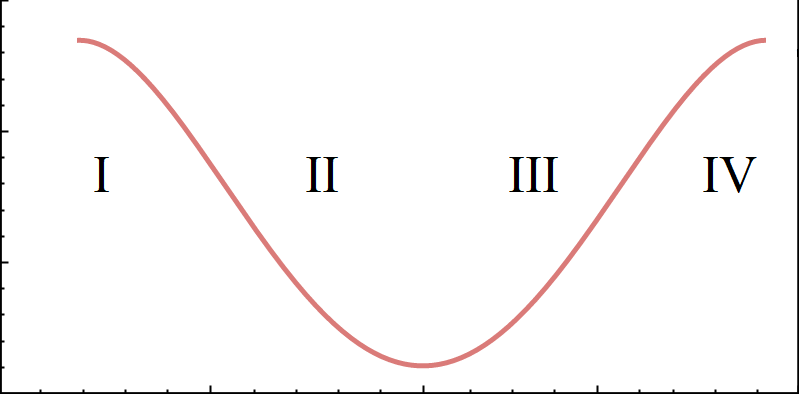
\includegraphics[width=0.5\textwidth]{../alt-ed-survey/figures-and-tables/figure-4.png}};
    %     \node (n2) [above=0.25cm] at ($(n1)!0.5!(n1) - (4, 1)$) {\rotatebox{90}{\textbf{Suitability}}};
    %     \node (n3) [above=0.25cm] at ($(n1)!0.5!(n1) - (0, 3)$) {\textbf{Time}};
    
    %     \end{tikzpicture}

    %     \label{fig:employer_driven_favorability}
    %     \end{figure}

    \section{Conclusions}

    % maybe talk about stress and debt for why debt is important
    % important to look at wages not income (which would include investments, etc, see shrm's discussion: http://www.cpepea.com/wp-content/uploads/2017/05/10-0418-Coalition-Report-on-Public-Policy-Issue-E-P-E-A_FNL.pdf)
    % SHRM assessed only a single year, 2008. Shows Section 127 is mostly a Master's degree tool rn.
    % 75 percentile for salaries in 2017 was 54250 https://bizfluent.com/info-10032733-percentile-salary.html
    % define middle class as 50-75 percentile, lower class as under 50 percentile. break down effect by salary classification and see if it helps lower/middle
    % if so, it should improve diversity of education leading to a more diverse workforce which employers crave (TM) and politicians, etc...
    % Should we actually enact this policy? Effect on alternative credentials and credential inflation
    % Other options like extending the benefit to repayment https://blog.shrm.org/blog/let-s-fight-the-skills-gap-by-expanding-tax-free-education-assistance
    % we can also consider extending the education benefit to unaccredited education and income share agreements not just loans
    
    % https://www.nber.org/papers/w9225.pdf 
    % https://www.nber.org/digest/feb03/w9225.html

    \bibliography{./BibFile}
    
    \end{document}
        